\documentclass[a4paper, 10pt]{article}
\usepackage[italian]{babel}
\usepackage[utf8]{inputenc}
\usepackage[T1]{fontenc}
\usepackage{amsthm, amsmath, amssymb}
\usepackage{graphicx}
\usepackage{geometry}
\geometry{margin=1in}
\usepackage{hyperref}
\usepackage{wrapfig}


\title{Advanced Deep Learning and Kernel Methods \\ Challenge 2}
\author{Valentinis Alessio\\Università degli Studi di Trieste}
\date{}

\begin{document}
\maketitle

\section{Introduction}
The goal of this challenge was to conduct an empirical analysis of the learnability of Neural Netwoks, in particular exploring the effect of the number of parameters
and on the capability of learning hierarchical functions.

\section{Source Code}
The complete code, including all experiments and implementation discussed in the following sections
is available at the following \href{https://github.com/ValentinisAlessio/Adv_DL_challenges}{GitHub repository}.

\section{Exercise A: The effect of \textit{under-} and \textit{over-}parametrization in the Teacher/Student setup}
The objective of this exercise was to train a Neural Network supervisedly on input/output pairs generated from a Neural Network with frozen archietecture and 
weights, called Teacher. In particular we were interested in the effect of the number of parameters of the Student on the learning process.

\subsection{Experimental Setup}
The Teacher was a simple feedforward Neural Network with 3 hidden layers of dimension 74, 50, 10 with ReLU activation functions. Te network takes as input 100-dimensional 
vetors and outputs a scalar value. Weights and biases were initialized as \textit{i.i.d.} samples from a Standard Normal distribution.

The Students on the other end, were of three kinds:
\begin{itemize}
    \item \textbf{Underparametrized}: a feedforward Neural Network with 1 hidden layers of dimension 10, with ReLU activation functions.
    \item \textbf{Equally parametrized}: identical to the Teacher.
    \item \textbf{Overparametrized}: a feedforward Neural Network with 4 hidden layers of dimension 200, 200, 200, 100 with ReLU activation functions.    
\end{itemize}

The training was done using the following procedure:
\begin{enumerate}
    \item Generate a test set of $6 \times 10^4$ samples from the Teacher, taking as input 100-dimensional vectors of i.i.d. samples from a Multivariate
    Uniform distribution in $[0, 2]^{100}$.
    \item Train each network on MSE loss on 1000 epochs, harvesting for each sample a fresh batch of 128 samples from the Multivariate Uniform distribution and
    obtaining the target by passing them through the Teacher. Adam optimizer was used, with a learning rate selected on a grid search $[5 \times 10^{-4}, 5\times 10 ^{-3}, 3.5\times 10^{-2}, 1\times 10^{-2}, 2\times10^{-1}]$
    and the best one was selected based on the validation loss.
    \item Evaluate the performance of the Student on the test set and harvest the weights and biases.
\end{enumerate}

\subsection{Results}
\subsubsection{Performance evaluation}
After performing some hyperparameter tuning, the best learning rate found were:
\begin{itemize}
    \item \textbf{Underparametrized}: 1
    \item \textbf{Equally parametrized}: 0.035
    \item \textbf{Overparametrized}: 0.035
\end{itemize}

The results of the training process are reported in the following figure:
\begin{figure}[h]
    \centering
    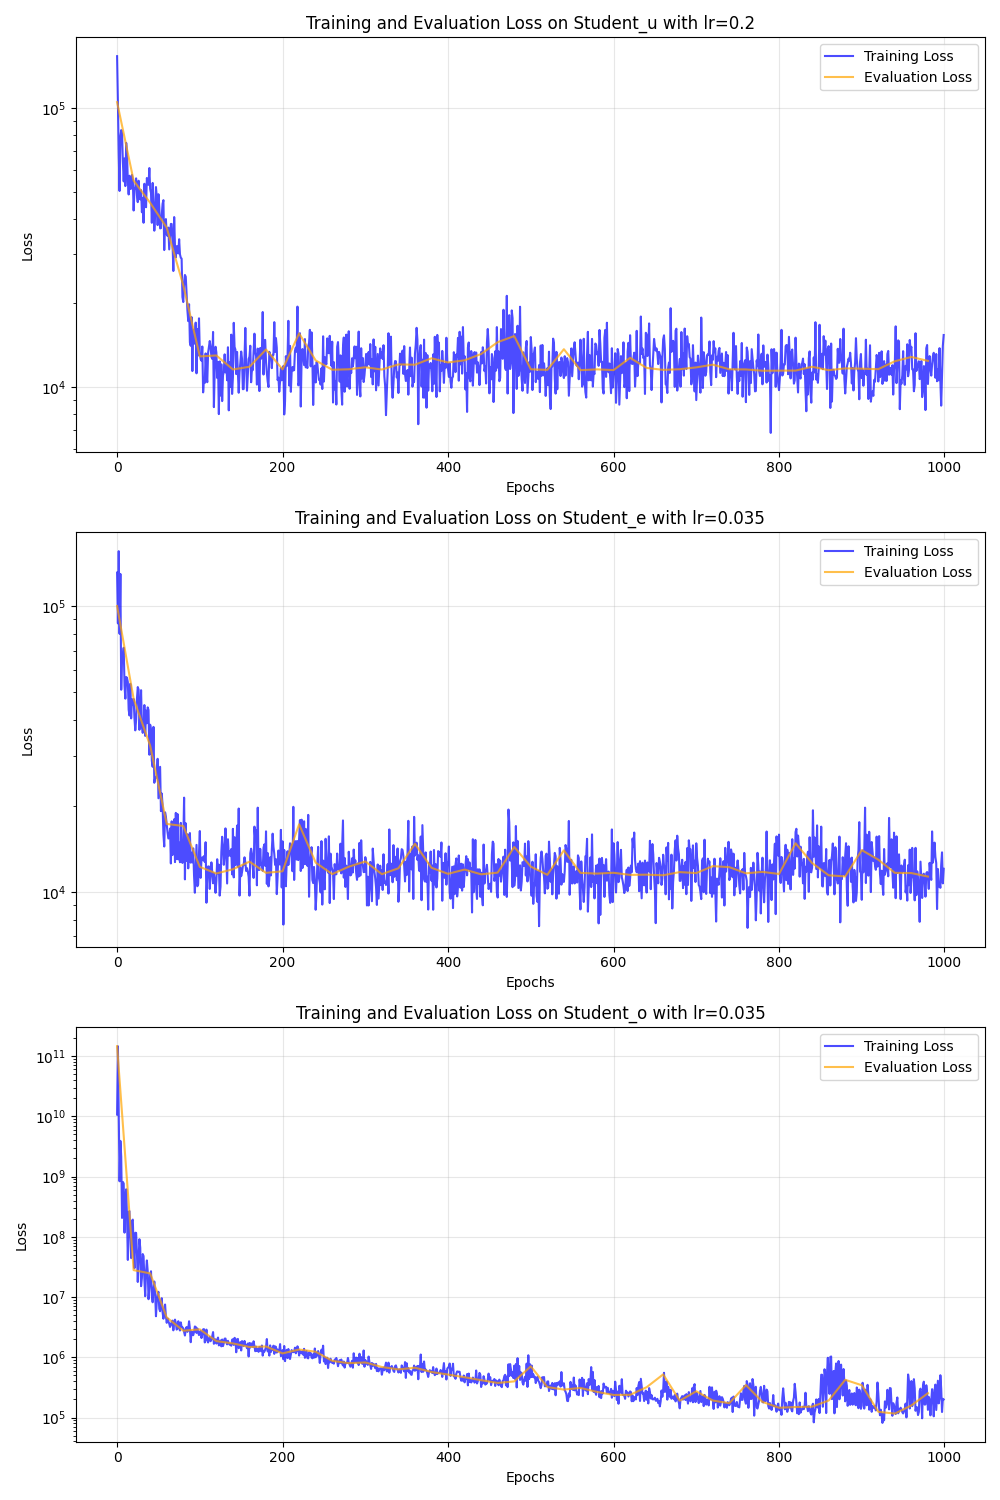
\includegraphics[width=0.5\textwidth]{images/training_curves_exA.png}
    \caption{Training curves of the Students}
    \label{fig:training_curves_exA}
\end{figure}

After training process, the performance of the Students on the test set was evaluated and the results are reported in the table below:
\begin{center}
    \begin{tabular}{c|c|c}
        \textbf{Student} & \textbf{Training Loss} & \textbf{Test Loss} \\
        \hline
        Underparametrized & 13496.06 & 11752.7 \\
        Equally parametrized & \textbf{11804.85} & 14566.2 \\
        Overparametrized & 12928.31 & \textbf{10965.8} \\
    \end{tabular}
    \label{tab:students_performance}
\end{center}

From this table we can observe how the best \textit{in-sample} performance was obtained by the equally parametrized Student, while the best \textit{out-of-sample} 
performance was obtained by the overparametrized Student. The underparametrized Student, on the other hand, performed poorly in both cases.

This behavior can be interpreted as an empyrical evidence of the \textit{double descent} phenomenon:
\begin{itemize}
    \item \textbf{Underparametrization regime}: the underparametrized student is not able to learn the target function, as the capacity of the model is
    not enough to capture the complexity of the function.
    \item \textbf{Interpolation regime}: the equally parametrized student is able to learn the target function in the training set, but it generalizes worse than
    the underparametrized student, as it is more prone to overfitting.
    \item \textbf{Overparametrization regime}: the overparametrized student is able to learn the target function in the test set, as it has enough capacity to
    both capture the complexity of the function and generalize well.
\end{itemize}

\subsubsection{Parameters distributions}
The next step was to analyze the distribution of the weights and biases of all the models and compare them, in order to understand how the number of parameters
affects the parameter values. This analysis was performed both globally and layer-wise.

\begin{figure}[h]
    \centering
    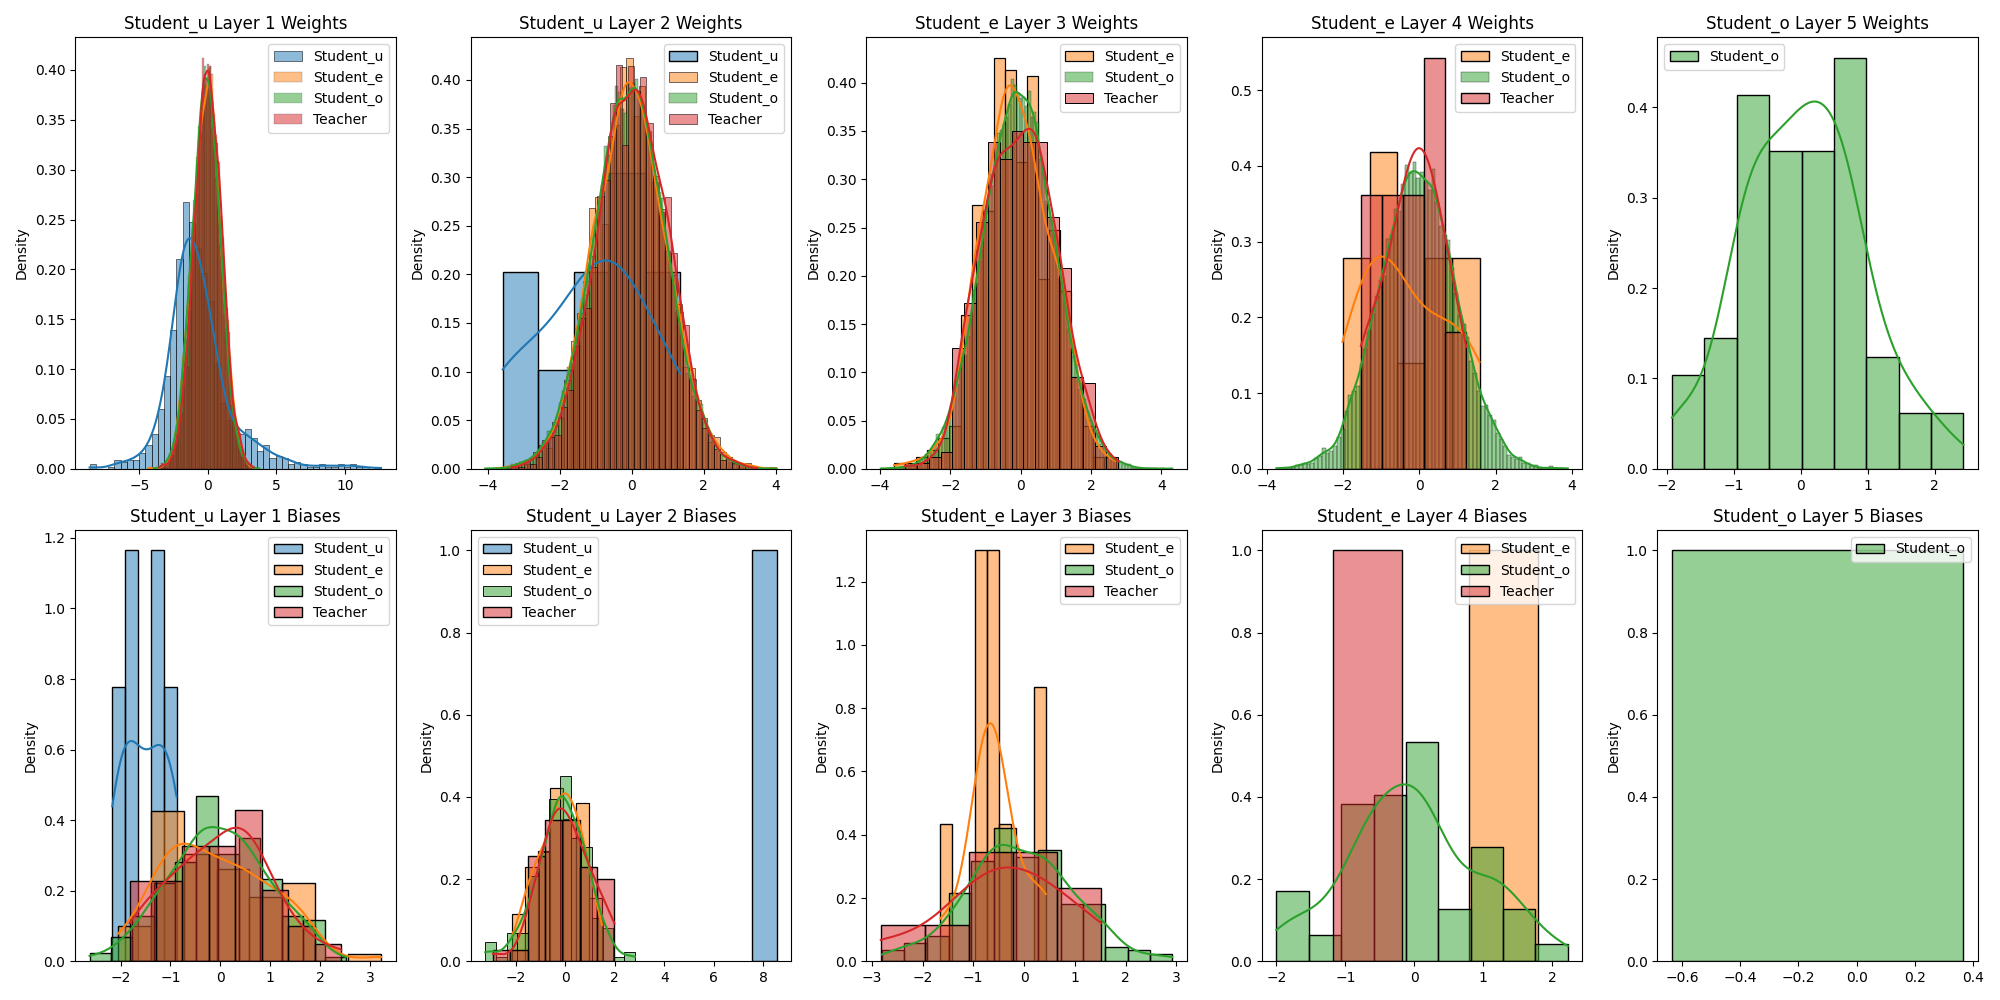
\includegraphics[width=0.7\textwidth]{images/weights_biases_histograms_layers_exA.png}
    \caption{Parameters distribution of the Students}
    \label{fig:weights_biases_histograms_layers_exA}
\end{figure}

From the histograms in \ref{fig:weights_biases_histograms_layers_exA}, we can see how the underparametrized Student has the worst-reflecting distribution compared to the Teacher, again supporting the 
hypothesis that the model is not able to learn properly the target function. The equally parametrized Student and the overparametrized one have a more similar
distribution, with the overparametrized one having a slightly more peaked distribution.

\begin{figure}[h]
    \centering
    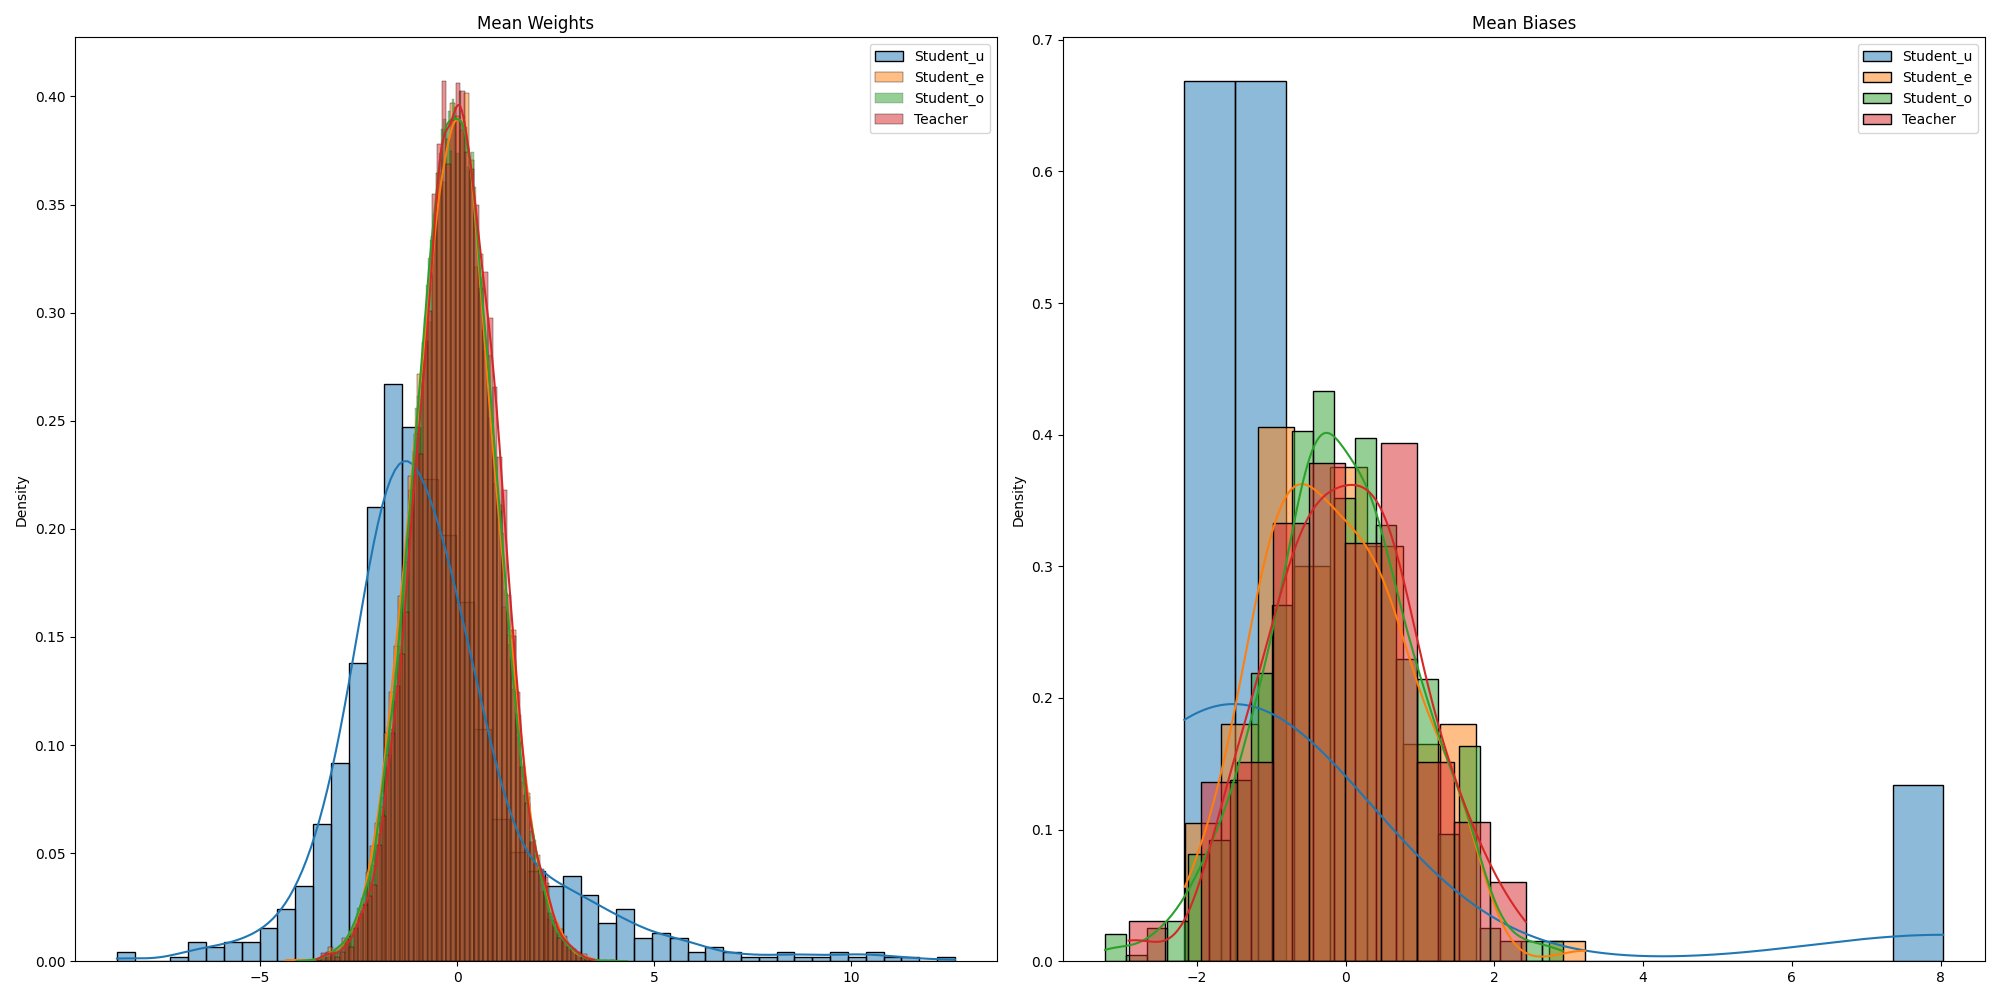
\includegraphics[width=0.5\textwidth]{images/weights_biases_histograms_global_exA.png}
    \caption{Parameters distribution of the Students}
    \label{fig:weights_biases_histograms_global_exA}
\end{figure}

From the histograms in \ref{fig:weights_biases_histograms_global_exA} we can observe how globally the distribution of the parameters of the underparametrized Student
are the most different from the Teacher, while concerning the other two models the distribution is more similar.


\section{Exercise B: Function learning and hierarchical functions}
The objective of this exercise was to train a deep residual neural network supervisedly on examples generated from specific polynomials. Although looking at the
monomials of these two polynomials they may seem very similar, the functions are actually very different, as the first one is the Bell polynomial of degree 6,
a hierarchical function, while the second one is obtained by randomly permute the indexes of each monomial independently. The formulation of the two polynomials is
the following:

\begin{align*}
    B_6(x_1, x_2, x_3, x_4, x_5, x_6) &= x_1^6 + 15x_2x_1^4 + 20x_3x_1^3 + 45x_2^2x_1^2 + 15x_2^3 + 60x_3x_2x_1 + 15x_4x_1^2 + \\
        & \quad + 10x_3^2 + 15x_4x_2 + 6x_5x_1 + x_6\\
    &= \sum_{i = 0}^{5}\left(\binom{5}{i} \right)B_{5-i}(x_1, \dots, x_{5-i})x_6\\
    \tilde{B_6}(x_1, x_2, x_3, x_4, x_5, x_6) &= x_3^6 + 15x_3x_2^4 + 20x_4x_2^3 + 45x_4^2x_3^2 + 15x_5^3 + 60x_4x_2x_5 + 15x_6x_5^2 + \\
        & \quad + 10x_2^2 + 15x_6x_4 + 6x_2x_5 + x_1
\end{align*}

\subsection{Experimental Setup}
The main part of the challenge consisted in training a deep ResNet, but first, we had to generate the training and test set. 
They were simply harvested by taking as input 6-dimensional vectors of i.i.d. samples from a Multivariate Uniform distribution in $[0, 2]^{6}$ and
the corresponging targets were obtained by passing them through the two polynomials. The training set was composed of $10^5$ samples, while the test set
was composed of $6\times 10^4$ samples. A total of two training sets and two test sets were generated, one for each polynomial.

The ResNet was composed of 9 hidden layers, each of dimension 50, with ReLU activation functions. The network takes as input 6-dimensional vectors and outputs
a scalar value. 

The training was done on the following parameters:
\begin{enumerate}
    \item Adam optimizer with a learning rate of $1\times 10^{-3}$ (selected from a grid search with the aim of minimizing the train loss).
    \item MSE loss on 50 epochs, with batches of 20 samples.
\end{enumerate}

After the training was completed, a final evaluation was done on the test set, and corresponding loss values were harvested.

After this process, a last process had to be performed, i.e.:
\begin{itemize}
    \item Sample a brand new test vector from the Multivariate Uniform distribution.
    \item For each of the components of the vector, evaluate both teh polynomials and the trained ResNets on a fine grid centered in that component.
    \item Keep track of the results and the errors.
\end{itemize}

\subsection{Results}
The results of the training process are reported in the following figure:
\begin{figure}[h]
    \centering
    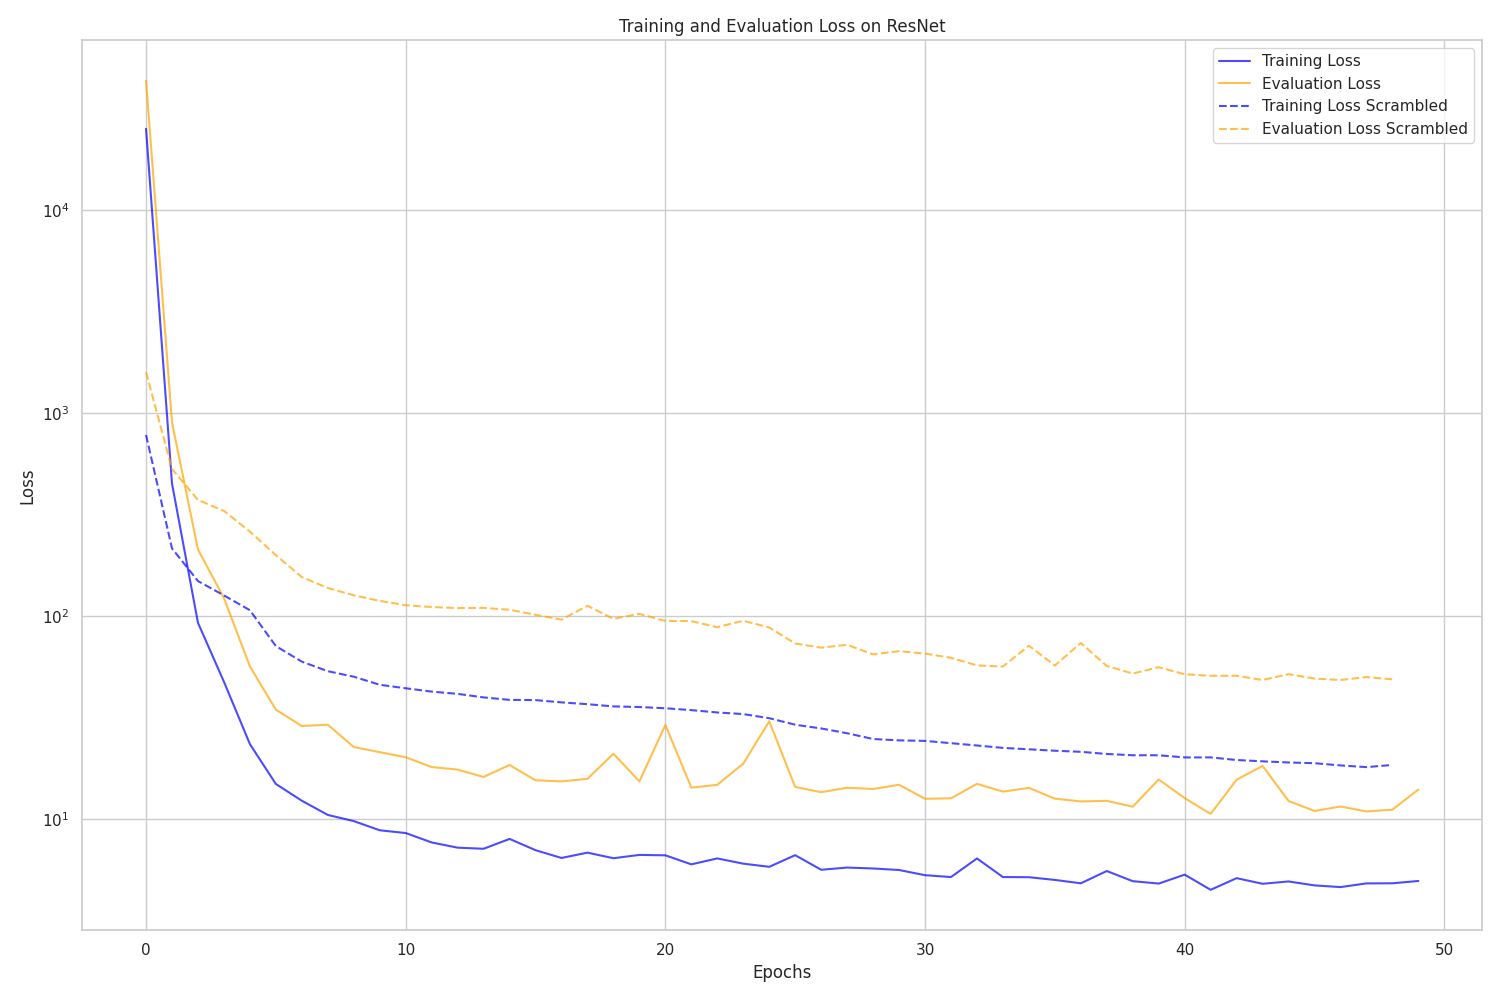
\includegraphics[width=0.6\textwidth]{images/training_curves_resnet_exB.png}
    \caption{Training curves of the ResNets}
    \label{fig:training_curves_resnet_exB}
\end{figure}

After the training process, the performance of the ResNets on the test set was evaluated and the results are reported in the table below:
\begin{center}
    \begin{tabular}{c|c}
        \textbf{Polynomial} & \textbf{Test Loss} \\
        \hline
        $B_6$ & 1.74656 \\
        $\tilde{B_6}$ & 16.9151 \\
    \end{tabular}
    \label{tab:resnets_performance}
\end{center}

Looking both at the training curves and the test loss values, we can see how the same archietecture is more capable of learning the hierarchical function $B_6$,
as its recursive formulation better resembples the architecture of the ResNet. This is not only reflected in the test loss, which is by far lower in the net trained
on $B_6$, but also in the training curves, where the net trained on $B_6$ converges faster and to a lower value.

The last part of the challenge was to evaluate the ResNets on a fine grid centered in a new test vector. The results are reported in the following figure:

\begin{figure}[h]
    \centering
    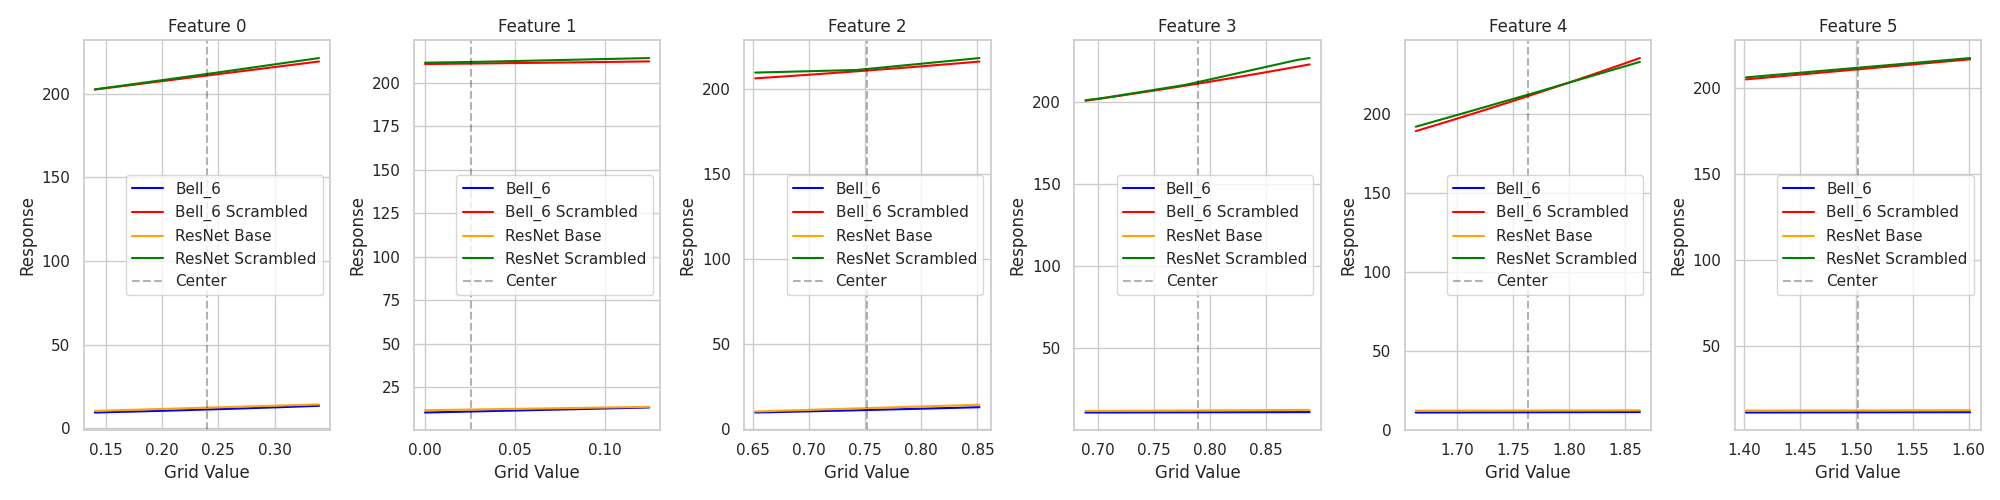
\includegraphics[width=0.8\textwidth]{images/predictions_exB.png}
    \caption{Fine grid evaluation of the ResNets}
    \label{fig:fine_grid_evaluation_exB}
\end{figure}

From this plot only not many information can be extracted, as the results yielded from the two polynomials and the corresponding ResNets are on differentscales, 
making interpretation not that straightforward. However, we can see how the ResNet trained on $B_6$ is able to better approximate the target function, as the
solutions are better overlapped.

\begin{figure}[h]
    \centering
    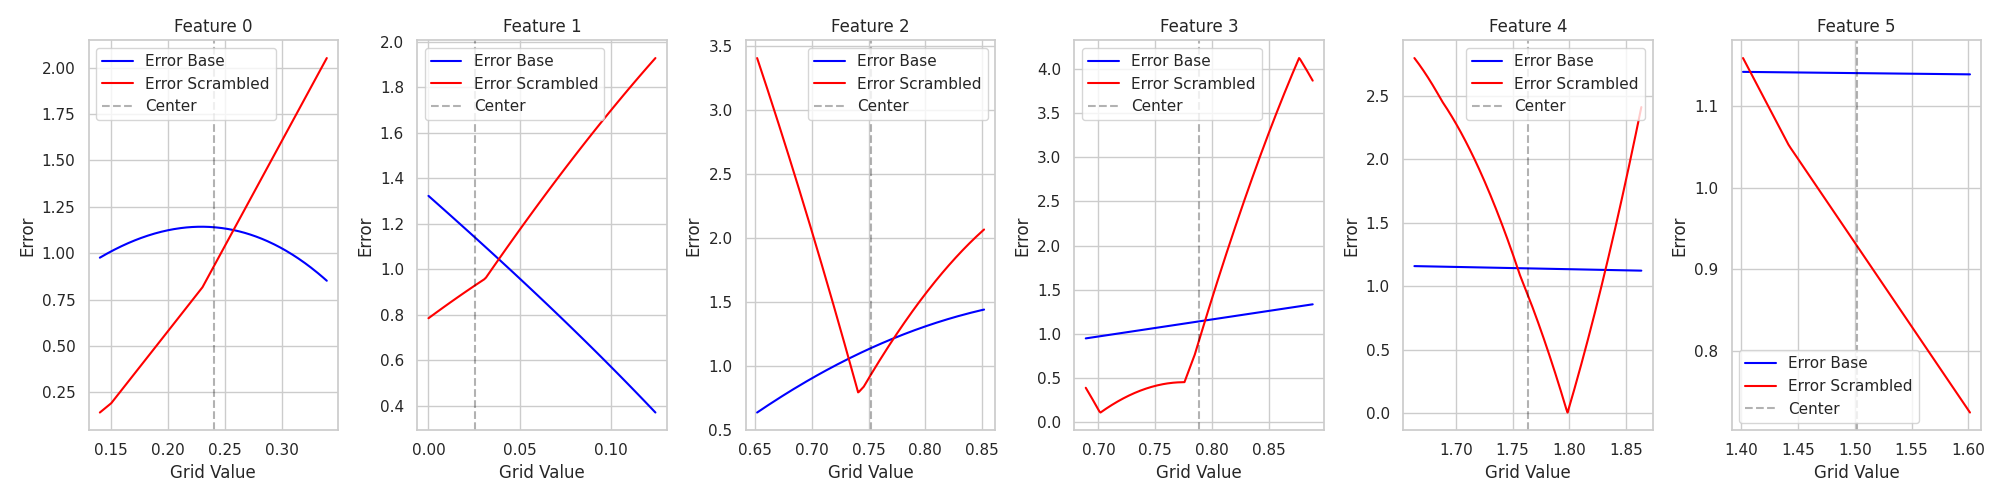
\includegraphics[width=0.8\textwidth]{images/errors_exB.png}
    \caption{Errors of the ResNets on the fine grid}
    \label{fig:errors_exB}
\end{figure}

If we instead look at the errors, we can see how the ResNet trained on $B_6$ has a lower and more constant error on the evaluation grid, for almost all the components
of the input vector, while the ResNet trained on $\tilde{B_6}$ has a higher and highly variable error. This is another empirical evidence that the ResNet trained
on the original hierarchical function is able to not only learn the target function better, but also generalize better, while the other ResNet looks like it is
overfitting the training set.

\section{Conclusions}
In this challenge we have explored the learnability capabilities of Neural Networks, in particular focusing on the effect of the number of parameters and their ability 
to learn hierarchical functions. In particular we have seen empirically the well-known \textit{double descent} phenomenon, where the best generalization performance
is obtained by the overparametrized model, and the importance of the architecture of the model in learning hierarchical functions.

Furthermore, we have seen how the same architecture can perform very differently on two similar functions, depending on the structure of the functions themselves.
Moreover we have seen how a resnet can learn properly the bell polynomial, being able to generalize well on a fine grid evaluation, while it is not the case for a
randomly permuted version of the same polynomial.

\end{document}